\documentclass[tikz,convert={outfile=\jobname.svg}]{standalone}
%\usetikzlibrary{...}% tikz package already loaded by 'tikz' option
\usepackage{amsmath,amssymb}  % Pour les symboles mathématiques
\usepackage{lmodern}          % Utilisation de la police lmodern pour meilleure compatibilité SVG
\usetikzlibrary{matrix,positioning}
\usetikzlibrary{arrows.meta}

\begin{document}


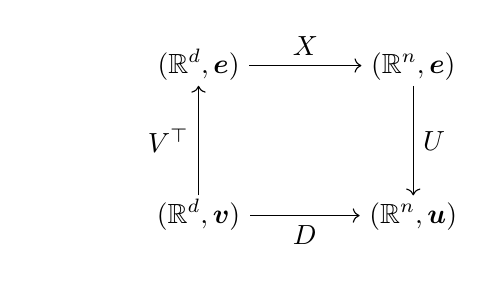
\begin{tikzpicture}
  \matrix (m) [matrix of math nodes, row sep=2em, column sep=4em, text height=1.5ex, text depth=0.25ex]
  {
    & (\mathbb{R}^d, \boldsymbol{e})  & (\mathbb{R}^n, \boldsymbol{e}) \\
    & & \\
    & (\mathbb{R}^d, \boldsymbol{v}) & (\mathbb{R}^n, \boldsymbol{u}) \\
  };

  % Flèches entre les cellules
  \path[->] (m-1-2) edge node[above] {$X$} (m-1-3);
  \path[->] (m-3-2) edge node[left] {$V^\top$} (m-1-2);
  \path[->] (m-1-3) edge node[right] {$U$} (m-3-3);
  \path[->] (m-3-2) edge node[below] {$D$} (m-3-3);
  
\end{tikzpicture}

% 
% \begin{tikzpicture}% Example:
%   \matrix (m) [matrix of math nodes, row sep=2em, column sep=4em, text height=1.5ex, text depth=0.25ex]
%   {
%     \mathbf{X} :& (\mathbb{R}^d, \boldsymbol{e})  & (\mathbb{R}^n, \boldsymbol{e}) \\
%     & & \\
%     & (\mathbb{R}^d, \boldsymbol{v}) & (\mathbb{R}^n, \boldsymbol{u}) \\
%   };
% 
%   % Arrows
%   \path[->] (m-1-2) edge node[above] {$V^\top$} (m-3-1)
%             % (m-2-2) edge node[above] {$D$} (m-2-3)
%             % (m-2-3) edge node[above] {$U$} (m-2-4);
% 
%   % Labels for spaces
%   \node[above of=m-1-2, node distance=1.5em] {Input Space $\mathbb{R}^d$};
%   \node[above of=m-1-3, node distance=1.5em] {Output Space $\mathbb{R}^n$};
% 
% \end{tikzpicture}
\end{document}